\date{}
\title{}
\date{}
\begin{document}
\begin{frame}
    \titlepage
\end{frame}


\section{last time}
\begin{frame}
\frametitle{last time}
\begin{itemize}
    \item routes via Dijkstras (best-first search)
    \item convergence time for distance vector v link-state
    \item OSPF areas --- distance vector with link-state
        \begin{itemize}
        \item goal: routers avoid tracking whole huge network
        \item no-loop rules: no going through areas except backbone
        \item exception: explicitly configured virtual links to backbone
        \end{itemize}
    \item interdomain routing
        \begin{itemize}
        \item business constraints --- someone needs to pay for traffic
        \item choosing routes by business priorities? (cost, performance, \ldots)
        \end{itemize}
\end{itemize}
\end{frame}

\section{interdomain routing}

\subsection{relationship types}
\begin{frame}{relationship types}
    \begin{itemize}
    \item provider/customer
        \begin{itemize}
        \item typically: customer pays provider
        \item provider connects customers everywhere it can (customer paid for it)
        \item customer does \textbf{not} provide paths through its network
        \end{itemize}
    \item peer/peer
        \begin{itemize}
        \item often: no payment (`settlement-free')
        \item if A peers with B\ldots
        \item A gets connected to B's customers (customers paid B for this)
        \item A does not get connected to B's other peers (no one paid B for this)
        \item A does not get connected to B's providers (no one paid B for this)
        \end{itemize}
    \end{itemize}
\end{frame}


\subsection{aside: connecting big networks}
\begin{frame}{connecting big networks?}
    \begin{itemize}
    \item some options:
        \begin{itemize}
        \item (which are basically the same as connecting parts of big network)
        \end{itemize}
    \vspace{.25cm}
    \item run a fiber between two buildings
        \begin{itemize}
        \item permitting and construction needed
        \end{itemize}
    \item pay for direct access to fiber someone else ran (``dark fiber'')
        \begin{itemize}
        \item burying one fiber costs similar to burying bundle, so spares
        \end{itemize}
    \item pay a telecom for a site-to-site connection
        \begin{itemize}
        \item ``gaurenteed'' bandwidth+latency between two sites
        \item may or may not use series of dedicated fibers
        \end{itemize}
    \item get space in common datacenter, pay datacenter operator for connection 
    \end{itemize}
\end{frame}


\subsection{local/remote preferences}
\usetikzlibrary{shapes,shapes.misc,arrows.meta,fit}

\begin{frame}{going the distance}
\begin{tikzpicture}
\tikzset{
    network/.style={draw,cloud,very thick,aspect=2},
    router/.style={draw,circle,fill=white},
    connect/.style={draw,ultra thick,Latex-Latex,black!50},
    send money/.style={bend right,draw,line width=1mm,green!70!black,dotted,"\huge\$",-Latex},
    every label/.style={font=\small},
}
\node[router,label={north:ISP A/Tokyo}] (A-japan) at (0, 1) {};
\node[router,label={south:ISP B/Tokyo}] (B-japan) at (0.5, -1) {};
\node[router] (A-japan-other) at (1.75, 0.75) {};
\node[router,label={north:ISP A/Los Angeles}] (A-la) at (6.5, .5) {};
\node[router,label={south:ISP B/Los Anegles}] (B-la) at (6.5, -1.5) {};
\node[router] (B-us-other) at (8.5, -1.25) {};
\node[router,label={north:ISP A/NoVA}] (A-va) at (10.5, 1.5) {};
\node[router,label={south:ISP B/NoVA}] (B-va) at (10.5, -.5) {};

\node[network,overlay] (jp-net) at (-1.5, 1) {};
\node[network,overlay] (va-net)at (13, -.5) {};
\foreach \x/\y in {A-japan/B-japan,A-la/B-la,A-va/B-va,A-japan/A-japan-other,A-japan-other/A-la,A-la/A-va,
                   B-japan/B-la,B-la/B-us-other,B-us-other/B-va,
                   va-net/B-va,jp-net/A-japan} {
    \draw[connect] (\x) -- (\y);
}
\begin{visibleenv}<2>
    \foreach \x/\y in {B-va/A-va,A-va/A-la,A-la/A-japan-other,A-japan-other/A-japan} {
        \draw[red,line width=1.5mm,solid,-Latex] (\x) -- (\y);
    }
    \foreach \x/\y in {B-va/B-us-other,B-us-other/B-la,B-la/B-japan,B-japan/A-japan} {
        \draw[blue,line width=1.5mm,dash dot dot,-Latex] (\x) -- (\y);
    }
    \foreach \x/\y in {va-net/B-va,A-japan/jp-net} {
        \draw[violet,line width=1.5mm,dashed,-Latex] (\x) -- (\y);
    }
    \node[align=left,very thick,draw=red,ultra thick,anchor=north] at (6, -3) {
        does ISP A or ISP B help packets cross the Pacific?
    };
\end{visibleenv}
\end{tikzpicture}
\end{frame}

\begin{frame}{distance preferences}
    \begin{itemize}
    \item ISP B$\rightarrow$ISP A across the Pacific:
    \vspace{.5cm}
    \item for ISP B:
        \begin{itemize}
        \item cheaper to hand-off packet to ISP A as soon as possible
        \item more control over performance if handing off as late as possible
        \end{itemize}
    \item for ISP A:
        \begin{itemize}
        \item cheaper to require ISP B to hand-off packet as late as possible
        \item more control over performance if B sends as soon as possible
        \end{itemize}
    \item maybe part of ISP A and ISP B peering agreement
    \end{itemize}
\end{frame}



\subsection{sharing routes: BGP}
\begin{frame}{Border Gateway Protocol}
    \begin{itemize}
    \item protocol for sending routes between networks
    \item used whereever routers from different ASes connect
    \vspace{.5cm}
    \item each router constructs list of routes to offer
        \begin{itemize}
        \item obtained from OSPF or similar
        \item route list filtered by administrator's policy
        \end{itemize}
    \item each router receives list of routes, exports
        \begin{itemize}
        \item sent as routes in OSPF or similar
        \item route list filtered by administrator's policy
        \end{itemize}
    \end{itemize}
\end{frame}

\begin{frame}{external/internal route sharing}
    \begin{itemize}
    \item AS wants to choose intelligently from all external options
    \item probably could do this with OSPF or similar, but\ldots
    \vspace{.5cm}
    \item usually have internal BGP instances (``iBGP'') to share this
        \begin{itemize}
        \item make sure every router knows all the ways out
        \end{itemize}
    \end{itemize}
\end{frame}


\subsection{BGP route format}
\begin{frame}{BGP route}
    \begin{itemize}
    \item adjacent routers share list of \textit{routes} with:
    \vspace{.5cm}
    \item IP prefix (CIDR-style, basically)
    \item AS path --- list of autonomous system the route goes through
    \item next hop router (IP address)
    \item \textit{multi-exit discriminator}
        \begin{itemize}
        \item low value = this entrance to AS is better than others for these IPs
        \end{itemize}
    \item \textit{local preference} (internal-only)
    \end{itemize}
\end{frame}

\begin{frame}{AS path}
    \begin{itemize}
    \item used to detect routing loops
    \vspace{.5cm}
    \item append your AS when sending route externally
    \item always ignore external routes with your AS in their AS path already
    \end{itemize}
\end{frame}


\subsection{sharing routes: picture}
\usetikzlibrary{arrows.meta,shapes}
\begin{frame}[fragile]{external BGP}
\begin{tikzpicture}
\tikzset{
    network/.style={draw,cloud,very thick,aspect=2,font=\fontsize{10}{11}\selectfont,align=center,inner sep=0.1mm},
    router/.style={draw,circle,fill=white},
    connect/.style={draw,ultra thick,Latex-Latex},
    send money/.style={bend right,draw,line width=1mm,green!70!black,dotted,"\huge\$",-Latex},
    bgp msg/.style={font=\fontsize{9}{10}\selectfont,fill=blue!5,align=left,draw,thick},
}
\node[network] (A) at (0,0) {ISP A\\\ldots\\AS64901};
\node[network] (B) at (4,0) {ISP B\\\ldots\\AS64895};
\node[network] (C) at (8,0) {ISP C\\\ldots\\AS64755};
\node[network] (D) at (12,0) {ISP D\\\ldots\\AS64600};
\node[network] (webhost) at (4,-5) {webhost \\3fff:1::/32\\AS64501};
\node[network] (office) at (8,-5) {office \\3fff:2::/32\\AS64502};
\node[network] (school) at (12, -5) {school \\3ff:7:ab::/40};
\draw[connect,alt=<2>{draw=red}] (A) -- (webhost);
\draw[connect,alt=<3>{draw=red}] (B) -- (webhost);
\draw[connect,alt=<4>{draw=red}] (C) -- (webhost);
\draw[connect,alt=<5>{draw=red}] (C) -- (D);
\draw[connect] (office) -- (B);
\draw[connect] (office) -- (D);
\draw[connect,alt=<6>{red}] (school) -- (D);
\begin{visibleenv}<2>
\path (A) -- (webhost) node[midway,bgp msg] {
    webhost$\rightarrow$A: \\
    \hspace{.5cm} 3fff:1::/32 () \\
    A$\rightarrow$webhost: \\
    \hspace{.5cm} \ldots
    \hspace{.5cm} \ldots
};
\end{visibleenv}
\begin{visibleenv}<3>
\path (B) -- (webhost) node[midway,bgp msg] {
    webhost$\rightarrow$B: \\
    \hspace{.5cm} 3fff:1::/32 () \\
    B$\rightarrow$webhost: \\
    \hspace{.5cm} 3fff::2::/32 (AS64502) \\
    \hspace{.5cm} \ldots
};
\end{visibleenv}
\begin{visibleenv}<4>
\path (C) -- (webhost) node[midway,bgp msg] {
    webhost$\rightarrow$C: \\
    \hspace{.5cm} 3fff:1::/32 () \\
    C$\rightarrow$webhost: \\
    \hspace{.5cm} 3fff::2::/32 (AS64502 AS64000) \\
    \hspace{.5cm} 3fff::7:ab::/40 (AS64000) \\
    \hspace{.5cm} \ldots
};
\end{visibleenv}
\begin{visibleenv}<5>
\path (office) -- (webhost) node[midway,bgp msg] {
    C$\rightarrow$D: \\
    \hspace{.5cm} 3fff:1::/32 (AS64501) \\
    \hspace{.5cm} \ldots \\
    D$\rightarrow$C: \\
    \hspace{.5cm} 3fff:2::/32 (AS64501) \\
    \hspace{.5cm} 3fff:7:ab::/32 () \\
    \hspace{.5cm} \ldots \\
};
\end{visibleenv}
\end{tikzpicture}
\end{frame}




\subsection{sharing routes: multiple connections}
\usetikzlibrary{arrows.meta,fit,shapes}

\begin{frame}[fragile]{multiple BGP sessions}
\begin{tikzpicture}
\tikzset{
    network/.style={draw,cloud,very thick,aspect=2,font=\fontsize{10}{11}\selectfont,align=center,inner sep=0.1mm},
    router/.style={draw,circle,fill=white},
    connect/.style={draw,ultra thick,Latex-Latex},
    send money/.style={bend right,draw,line width=1mm,green!70!black,dotted,"\huge\$",-Latex},
    bgp msg/.style={font=\fontsize{8}{9}\selectfont,fill=blue!5,align=left,draw=black,text=black,thick},
}
\node[router] (A-r1) at (-3, 0) {};
\node[router] (A-r2) at (3, 0) {};
\draw[connect] (A-r1) -- (-2, 1) node{\ldots};
\draw[connect] (A-r1) -- (-3.5, 1.8) node{\ldots};
\draw[connect] (A-r2) -- (2, 1.5) node{\ldots};
\draw[connect] (A-r2) -- (2.5, 2.5) node{\ldots};
\draw[connect] (A-r2) -- (1.2, 0.5) node{\ldots};
\node[router] (B-r1) at (-4, -2) {};
\node[router] (B-r2) at (5, -2) {};
\draw[connect] (B-r1) -- (-3, -4) node{\ldots};
\draw[connect] (B-r1) -- (-4, -5) node{\ldots};
\draw[connect] (B-r2) -- (4, -3) node{\ldots};
\draw[connect] (B-r2) -- (2, -2.5) node{\ldots};
\begin{pgfonlayer}{bg}
\node[fill=violet!10,fit={(A-r1) (A-r2) (2.5, 2.5) (-3.5, 1.8)}] {ISP A};
\node[fill=green!10,fit={(B-r1) (B-r2) (-3, -4) (-4, -5) (4, -3) (2, -2.5)}] {company B};
\end{pgfonlayer}
\begin{visibleenv}<2-3>
\draw[connect,red] (A-r1) -- (B-r1)
    node[midway,below right,bgp msg] {
        A$\rightarrow$B: \\
        \hspace{.5cm} 2601:db8:33::/40, MED=10 () \\
        \hspace{.5cm} 3fff:1234:99::/40, MED=10 (AS65432) \\
        \hspace{.5cm} 3fff:1234:abc::/40, MED=20 (AS65323) \\
        \hspace{.5cm} \ldots \\
        B$\rightarrow$A: \\
        \hspace{.5cm} 3fff:3230:10::/40, MED=20 () \\
        \hspace{.5cm} 3fff:3230:20::/40, MED=10 () \\
        \hspace{.5cm} \ldots
    };
\draw[connect,red] (A-r2) -- (B-r2)
    node[midway,above right,bgp msg] {
        A$\rightarrow$B: \\
        \hspace{.5cm} 2601:db8:33::/40, MED=30 () \\
        \hspace{.5cm} 3fff:1234:99::/40, MED=20 (AS65432) \\
        \hspace{.5cm} 3fff:1234:abc::/40, MED=10 (AS65823) \\
        \hspace{.5cm} \ldots \\
        B$\rightarrow$A: \\
        \hspace{.5cm} 3fff:3230:10::/40, MED=10 ()  \\
        \hspace{.5cm} 3fff:3230:20::/40, MED=20 () \\
        \hspace{.5cm} \ldots
    };
\end{visibleenv}
\begin{visibleenv}<3>
\node[draw=red,ultra thick,font=\small,align=left,fill=white] at ([xshift=.5cm,yshift=-1cm]B-r2.north east) {
    exchange possible routes \\
    over each pair of routers \\
    ~ \\
    typically same routes for \\
    each connection to AS \\
    but maybe different attributes 
};
\end{visibleenv}
\begin{visibleenv}<4->
\draw[connect] (A-r1) -- (B-r1);
\draw[connect] (A-r2) -- (B-r2);
\draw[dotted,red,very thick,Latex-Latex] (A-r1) -- (A-r2)
    node[midway,below=1cm,bgp msg] {
        left router$\rightarrow$all: \\
        \hspace{.5cm}via 3ff:3230:10::3, 3fff:3230:10::/40, MED=10 (AS64992) \\
        \hspace{.5cm}via 3ff:3230:10::3, 3fff:3230:20::/40, MED=20 (AS64992) \\
        \hspace{.5cm}\ldots \\
        right router$\rightarrow$all: \\
        \hspace{.5cm}via 3ff:3230:20::5, 3fff:3230:10::/40, MED=10 (AS64992) \\
        \hspace{.5cm}via 3ff:3230:20::5, 3fff:3230:20::/40, MED=20 (AS64992) \\
        \hspace{.5cm}\ldots \\
    };
\draw[dotted,red,very thick,Latex-] (A-r1) -- (2, 1.5) node[above]{\ldots};
\draw[dotted,red,very thick,Latex-] (A-r1) -- (-2, 1.75) node[above]{\ldots};
\draw[dotted,red,very thick,Latex-] (A-r2) -- (2, 1.5) node[above]{\ldots};
\draw[dotted,red,very thick,Latex-] (A-r2) -- (-2, 1.9) node[above]{\ldots};
\end{visibleenv}
\begin{visibleenv}<4>
\node[draw=red,ultra thick,font=\small,align=left,fill=white,anchor=north] at (8,-1) {
    within ISP, use internal BGP (IBGP) \\
    share everything learned via BGP \\
    with all BGP routers
};
\end{visibleenv}
\end{tikzpicture}
\end{frame}


\subsection{BGP route preference order}
\begin{frame}{preference between routes}
    \begin{itemize}
    \item if multiple choices, most common strategy:\ldots
    \item should use most specific route
        \begin{itemize}
        \item use 2001:db8:1234::/40 over 2001:db8:1234::/39 if both apply
        \item (but usually reject very small address ranges (e.g. /31 for IPv4, /60 for IPv6))
        \end{itemize}
    \item then (if tie) local policy applies
    \item then shortest AS path
    \item then lower AS number
    \item then (sometimes) lower MED (multiple exit discriminator)
    \item then best route within current AS
    \end{itemize}
\end{frame}

\begin{frame}[fragile]{multi-exit discriminator}
\begin{tikzpicture}
\tikzset{
    network/.style={draw,cloud,very thick,aspect=2},
    router/.style={draw,circle,fill=white},
    connect/.style={draw,ultra thick,Latex-Latex,black!50},
    send money/.style={bend right,draw,line width=1mm,green!70!black,dotted,"\huge\$",-Latex},
    every label/.style={font=\small},
}
\node[network,overlay] (jp-net-B) at (-1.5, 1) {2001:db8:1::/40};
\node[network,overlay] (va-net-A) at (13, -.5) {3fff:3:4::/40};
\node[router,label={north:ISP A/Tokyo}] (A-japan) at (0, 1) {};
\node[router,label={south:ISP B/Tokyo}] (B-japan) at (0.5, -1) {};
\node[router] (A-japan-other) at (1.75, 0.75) {};
\node[router,label={north:ISP A/Los Angeles}] (A-la) at (6.5, .5) {};
\node[router,label={south:ISP B/Los Anegles}] (B-la) at (6.5, -1.5) {};
\node[router] (B-us-other) at (8.5, -1.25) {};
\node[router,label={north:ISP A/NoVA}] (A-va) at (10.5, 1.5) {};
\node[router,label={south:ISP B/NoVA}] (B-va) at (10.5, -.5) {};
\foreach \x/\y/\med in {A-japan/B-japan/1,A-la/B-la/2,A-va/B-va/3} {
    \draw[connect] (\x) -- (\y);
    \draw[red] (\y) -- (\x) node[midway,fill=white,draw=red,align=left,font=\small] {
            to 2001:db8:1::/40, MED=\med
    };
}
\foreach \x/\y in {A-japan/B-japan,A-la/B-la,A-va/B-va,A-japan/A-japan-other,A-japan-other/A-la,A-la/A-va,
                   B-japan/B-la,B-la/B-us-other,B-us-other/B-va,
                   va-net/B-va,jp-net/A-japan} {
    \draw[connect] (\x) -- (\y);
}
\end{tikzpicture}
\end{frame}

\begin{frame}{getting your preference}
    \begin{itemize}
    \item to affect how people route you, can\ldots
    \vspace{.5cm}
    \item prepend to AS path sent to make it longer
        \begin{itemize}
        \item typically add serveral copies of your AS number
        \end{itemize}
    \item only announce network from certain of your routers
        \begin{itemize}
        \item problem: won't have all `backup' paths available
        \end{itemize}
    \item announce a large network in more specific pieces
        \begin{itemize}
        \item 3fff:1234::/32 as 3fff:1234::/33 and 3fff:1234:8000::/33
        \end{itemize}
    \item get other networks to change how they forward your routes
        \begin{itemize}
        \item often enabled through `BGP communities'
        \end{itemize}
    \end{itemize}
\end{frame}
 % FIXME: show multi-exit discriminator

\section{UVa, in practice}

\subsection{in practice?}
\begin{frame}[fragile]{}
    \begin{itemize}
    \item \url{https://bgp.he.net/super-lg/}
    \item \url{https://bgp.he.net/super-lg/#128.143.0.0/16?tob=none&mt=include&ma=6939&els=exact}
    \item \url{https://lg.ring.nlnog.net/prefix?q=128.143.0.0/16&match=exact&peer=all}
    \end{itemize}
\end{frame}

\begin{frame}{}
\url{https://bgp.he.net/AS225} (University of Virginia) \\
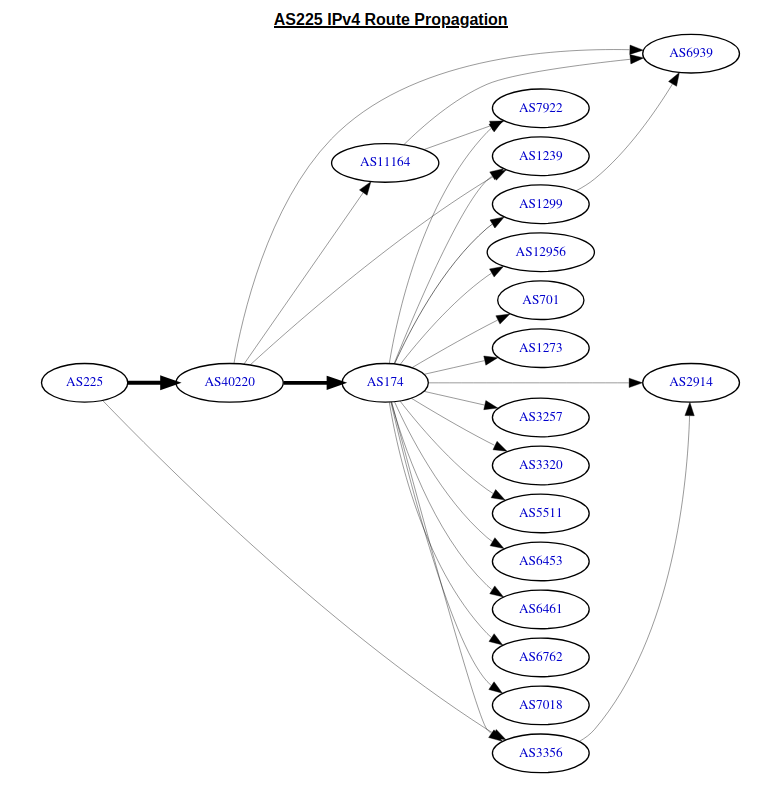
\includegraphics[width=0.5\textwidth]{../routing/as225-graph}
\end{frame}

\begin{frame}{AS40220}
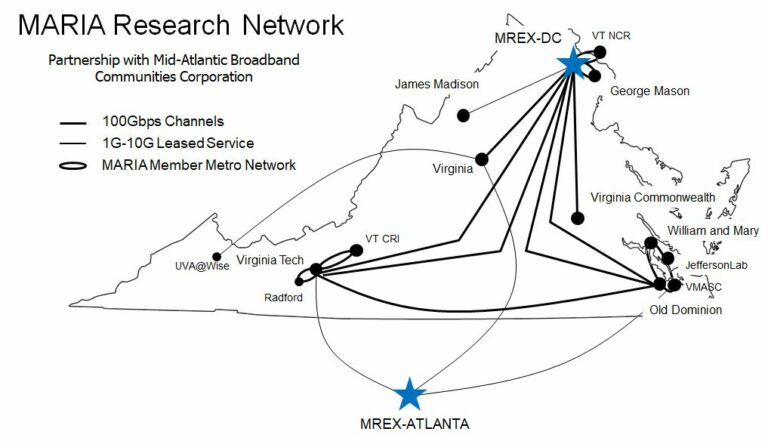
\includegraphics[height=0.8\textheight]{../routing/MARIA-Network-BW-768x441.jpg}
\end{frame}

\begin{frame}{}
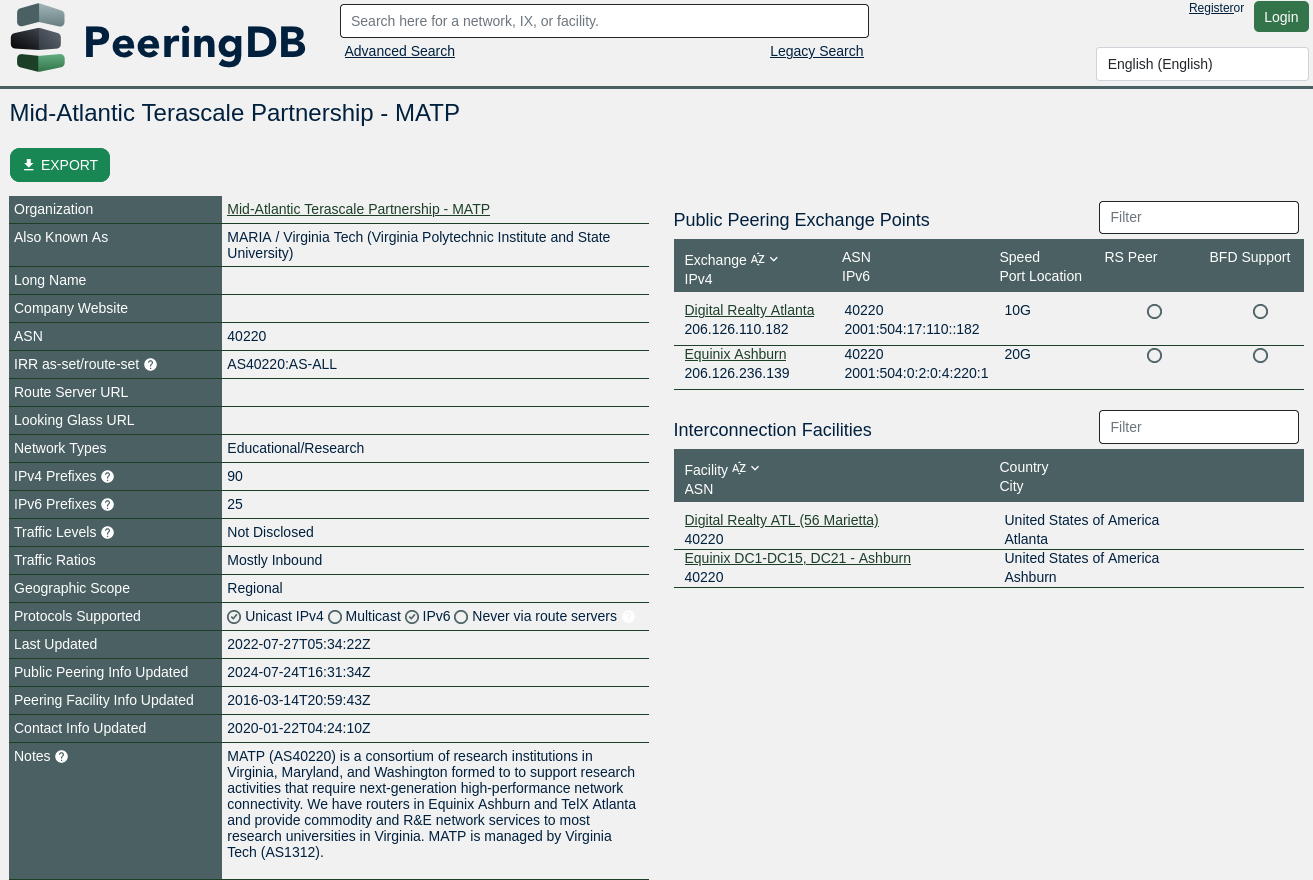
\includegraphics[width=0.95\textwidth]{../routing/as40220-peeringdb}
\end{frame}

\begin{frame}{AS3356}
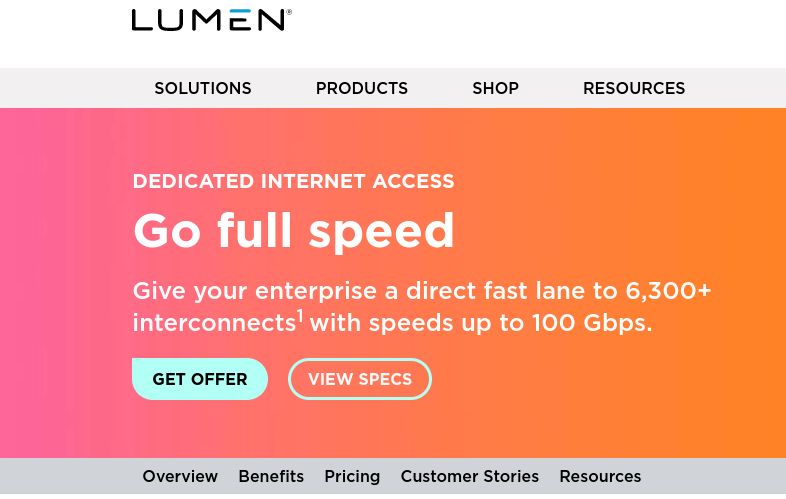
\includegraphics[height=0.8\textheight]{../routing/lumen-webpage.png}
\end{frame}

\begin{frame}{AS3356 is a backup (8x AS prepending)}
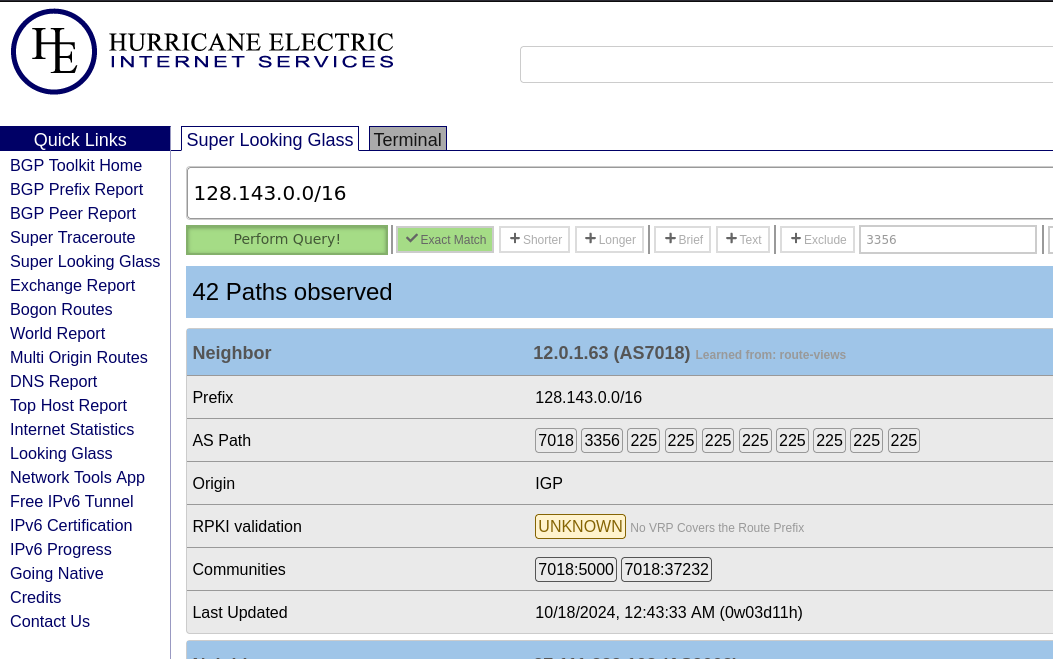
\includegraphics[height=0.8\textheight]{../routing/as3356-he-superlg.png}
\end{frame}


\subsection{internet exchanges, peeringdb}


\begin{frame}{peeringdb}
    \begin{itemize}
    \item \url{https://peeringdb.com} --- commonly used database of ASes and how to peer with them
    \item there is also -- ``whois'' records (from RIRs) for ASes, IP blocks with contact info
    \end{itemize}
\end{frame}

\begin{frame}{internet exchanges and route servers}
    \begin{itemize}
    \item internet exchange
        \begin{itemize}
        \item local network (typically within metro area) for connecting networks
        \item often run at and/or by `carrier-neutral' datacenter
        \item typically high bandwidth (10-100Gbps ports to network)
        \item provides connections when
        \end{itemize}
    \vspace{.5cm}
    \item route servers
        \begin{itemize}
        \item BGP servers run by internet exchange
        \item consolidates routes from participants
        \item goal: only need O($n$) BGP connections, not O($n^2$)
        \end{itemize}
    \end{itemize}
\end{frame}


\subsection{BGP communities}
\begin{frame}{BGP communities}
    \begin{itemize}
    \item routes sent via BGP can have `communities'
    \item extra information tagged on routes sent via BGP
    \vspace{.5cm}
    \item large ISPs have lists of communities their customers/peers can use
    \item \ldots and these affect how those routes are used
    \end{itemize}
\end{frame}

\begin{frame}{aside: Internet2}
    \begin{itemize}
    \item non-profit networking consortium
    \item operations major US University-focused network
    \item basically one of UVa's ISPs
    \end{itemize}
\end{frame}

\begin{frame}[fragile]{selected Internet2 BGP communities}
\begin{tikzpicture}
\node (a) {
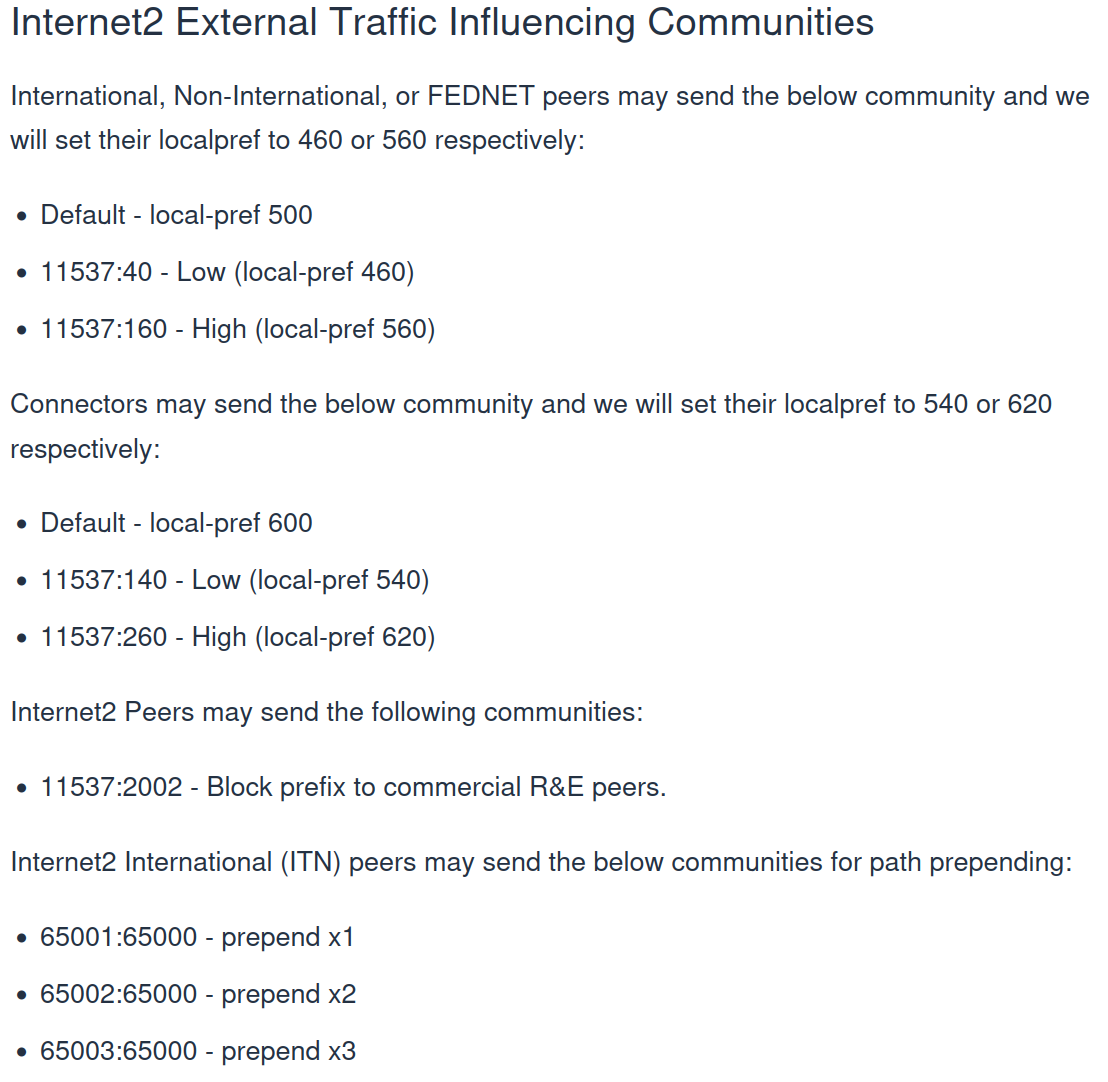
\includegraphics[width=0.49\textwidth]{../routing/i2-bgp-ext-comm}
};
\node[anchor=north west] (b) at (a.north east) {
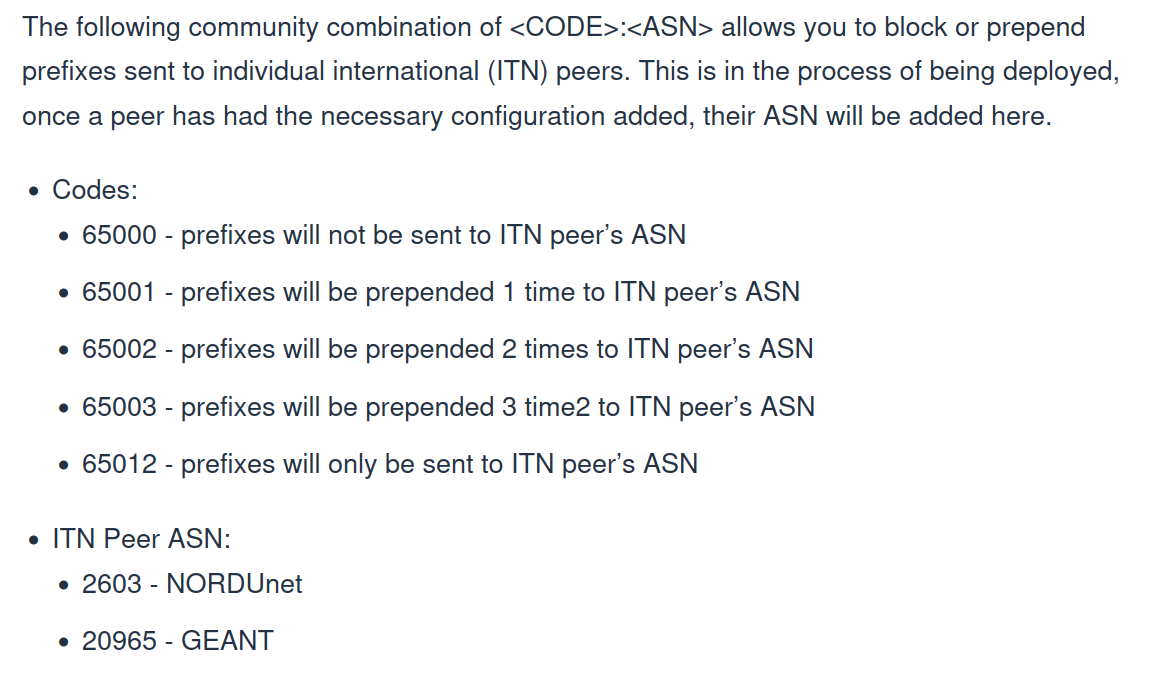
\includegraphics[width=0.39\textwidth]{../routing/i2-bgp-ext-comm2}
};
\node[anchor=north west] (c) at (b.south west) {
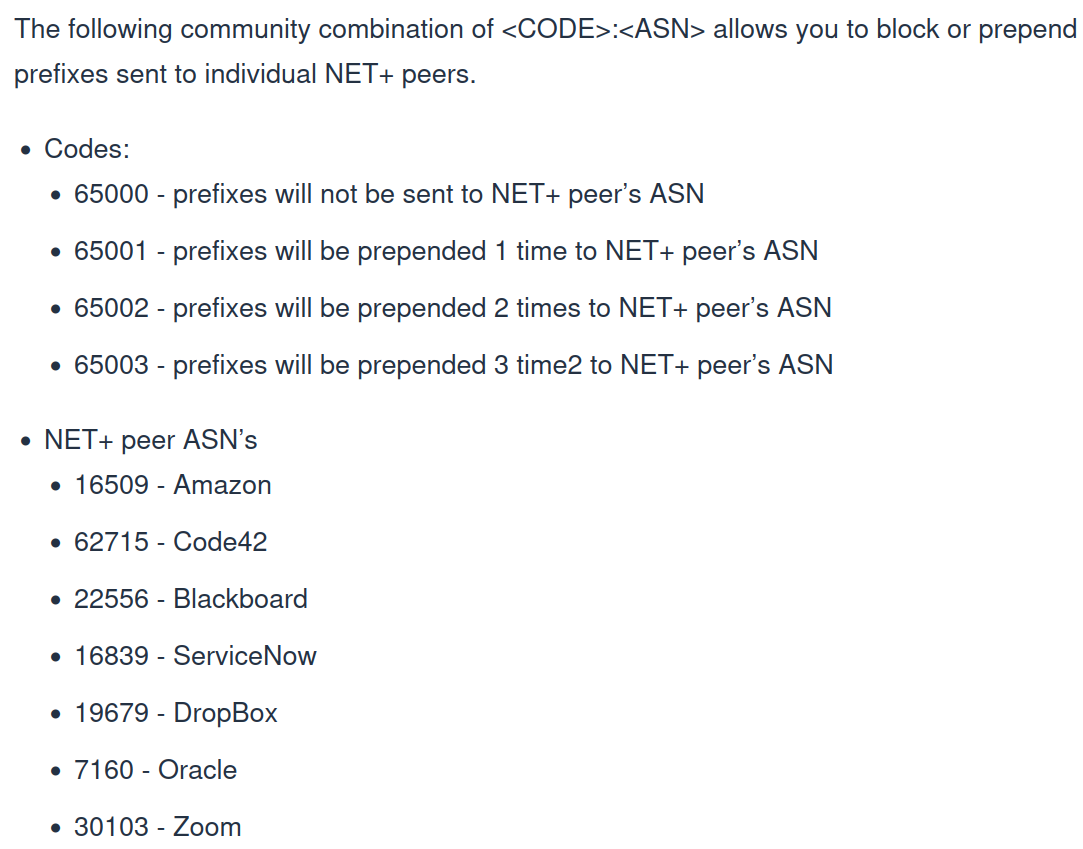
\includegraphics[width=0.39\textwidth]{../routing/i2-bgp-ext-comm3}
};
\end{tikzpicture}
{\fontsize{9}{10}\selectfont\url{https://noc.net.internet2.edu/knowledge/policy-statements/internet2-bgp-communities.html}}
\end{frame}

\begin{frame}{community options from prev slide}
\begin{itemize}
\item setting local-pref:
    \begin{itemize}
    \item you can decide how preferred your route is by Internet2
    \item maybe to make one primary, another secondary?
    \end{itemize}
\item blocking route from being sent to specific place
\item prepending Internet2's AS before forwarding prefix
    \begin{itemize}
    \item hopefully make that route less preferred by others
    \end{itemize}
\item prepending Internet2's AS before forwarding prefix to specific place
    \begin{itemize}
    \item hopefully make that route less preferred by that place
    \end{itemize}
\end{itemize}
\end{frame}

\begin{frame}{other things with communities}
    \begin{itemize}
    \item Internet2 also uses communities to mark\ldots
    \item what location routes were learned from
    \item what type of organization routes were learned from
    \item whether Internet2 is only allowed to use the route non-commerically or not
    \item \ldots
    \end{itemize}
\end{frame}



\subsection{BGP hijacking/fat fingers}

\begin{frame}{AS7007}
{\fontsize{8}{9}\selectfont\url{https://seclists.org/nanog/1997/Apr/444}}

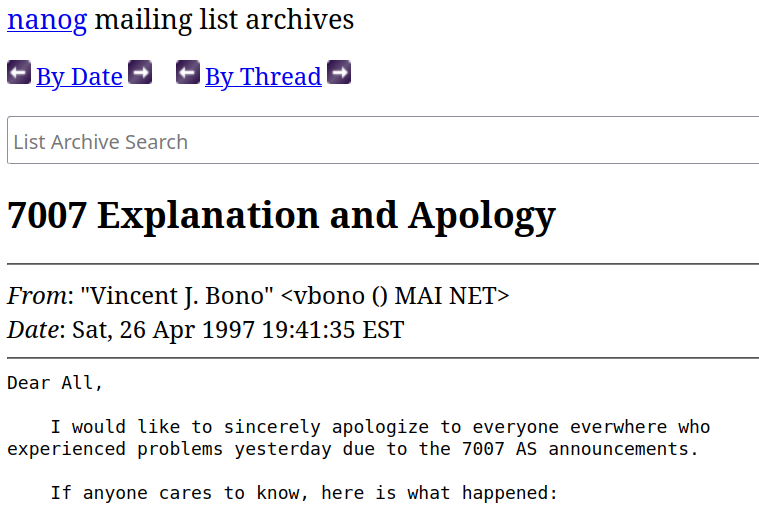
\includegraphics[width=0.4\textwidth]{../routing/as7007-1.png}
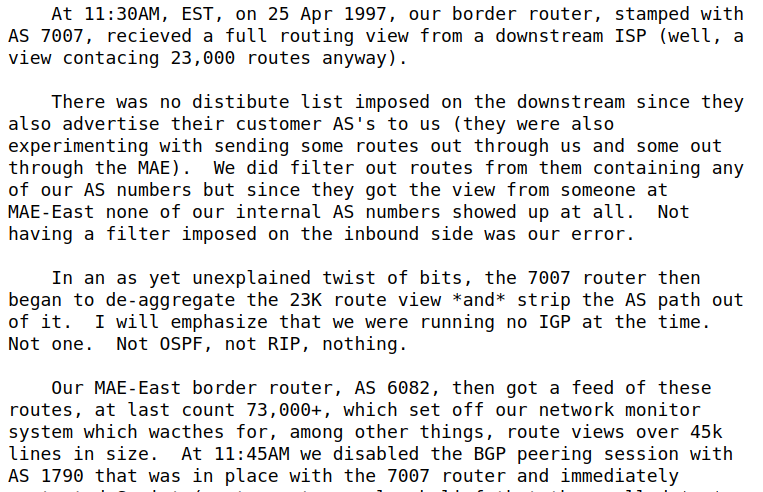
\includegraphics[height=0.4\textwidth]{../routing/as7007-2.png}
\end{frame}

\begin{frame}{2008 Pakistan Youtube}
\begin{itemize}
\item Pakistan Telecom recieved gov't order to block youtube
\item implemented by inserting route for YouTube's IP in internal network
\vspace{.5cm}
\item misconfiguration meant route was advertised on BGP
\item was more specific than YouTube's route, so made YouTube unreachablej
\end{itemize}
\end{frame}

\begin{frame}{timeline from RIPE NCC}
\begin{itemize}
\item {\tiny \url{https://www.ripe.net/about-us/news/youtube-hijacking-a-ripe-ncc-ris-case-study/}}
\item Youtube is announcing 208.65.152.0/22
\item 18:47Z: Pakistan Telecom starts announcing 208.65.153.0/24
\item 20:07Z: Youtube starts announcing 208.65.152.0/24
\item 20:18Z: Youtube starts announcing 208.65.152.0/25 and 208.65.152.128/25
\item 20:51Z: Pakistan Telecom's ISP forwards their announcements with additional copy of Pakistan Telecom's AS number
\item 21:01Z: Pakistan Telecom's ISP withdraws routes initiated by Pakistan Telecom (but not Pakistan Telecom's customers)
\end{itemize}
\end{frame}

\begin{frame}{BGP Hijacking targeted cryptocurrency stuff}
    \begin{itemize}
    \item KLAYswap (Feb 2022), Celer Bridge (Sep 2022)
    \item attackers intentionally redirected traffic to malicious version of services
    \item \ldots and stole money
    \vspace{.5cm}
    \item both probably spoofed the final AS number in AS path
    \item sometimes involved adding attacked IP range to routing registry
    \end{itemize}
\end{frame}

\begin{frame}{nation-states?}

\includegraphics[width=\textwidth]{../routing/china-tele-ars-tech}
\end{frame}


\subsection{validating routes / sBGP}
\begin{frame}{route security}
    \begin{itemize}
    \item historically, no verification routes announced by ``owner'' of IP addresses
    \vspace{.5cm}
    \item probably some ISPs filter
    \item effort to deploy RPKI --- public-key based scheme to verify routes
        \begin{itemize}
        \item checks that routes originated at correct AS
        \item doesn't verify intermediate ASes will forward correctly
        \end{itemize}
    \end{itemize}
\end{frame}

\begin{frame}{}
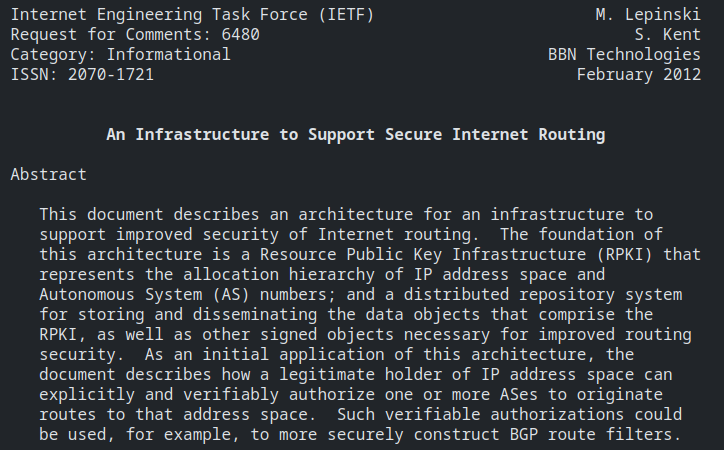
\includegraphics[height=\textheight]{../routing/rpki-rfc}
\end{frame}



\subsection{aside: partial tables}
\begin{frame}{partial tables}
    \begin{itemize}
    \item dealing with full Internet routing table is expensive
    \vspace{.5cm}
    \item common shortcut if you have a couple ISPs:
    \item keep `short' routes (example: short AS path)
    \item use default route for other cases
        \begin{itemize}
        \item to one of your ``primary'' ISPs
        \item maybe using ECMP
        \end{itemize}
    \end{itemize}
\end{frame}



\section{backup slides}
\begin{frame}\frametitle{backup slides}
\end{frame}

\end{document}
